%%%%%%%%%%%%%%%%%%%%%%%%%%%%%%%%%%%%%%%%%%%%%%%%%%%%%%%%%%%%%%%%%%%%%%%%%
%  Zawartość: Główny plik szablonu pracy dyplomowej (magisterskiej/inżynierskiej).
%  Opracował: Tomasz Kubik <tomasz.kubik@pwr.edu.pl>
%  Data: kwiecień 2016
%  Wersja: 0.2
%%%%%%%%%%%%%%%%%%%%%%%%%%%%%%%%%%%%%%%%%%%%%%%%%%%%%%%%%%%%%%%%%%%%%%%%%

\documentclass[a4paper,onecolumn,oneside,12pt,extrafontsizes]{memoir}
% W celu przygotowania wydruku do archiwum należy przesłonić komendę powyższą
% dwoma poniższymi komendami:
%\documentclass[a4paper,onecolumn,twoside,10pt]{memoir} 
%\renewcommand{\normalsize}{\fontsize{8pt}{10pt}\selectfont}

%\usepackage[cp1250]{inputenc} % jeśli kodowanie edytowanych plików to cp1250 
\usepackage[utf8]{inputenc} % jeśli kodowanie edytowanych plików to UTF8
\usepackage[T1]{fontenc}
\usepackage[polish]{babel}
%\DisemulatePackage{setspace}
\usepackage{setspace}
\usepackage{tabularx}
\usepackage{color,calc}
%\usepackage{soul} % pakiet z komendami do podkreślania tekstu
\usepackage{ebgaramond} % pakiet z czcionkami garamond, potrzebny tylko do strony tytułowej, musi wystąpić przed pakietem tgtermes

%% Aby uzyskać polskie literki w pdfie (a nie zlepki) korzystamy z pakietu czcionek tgterms. 
%% W pakiecie tym są zdefiniowane klony czcionek Times o kształtach: normalny, pogrubiony, italic, italic pogrubiony.
%% W pakiecie tym brakuje czcionki o kształcie: slanted (podobny do italic). 
%% Jeśli w dokumencie gdzieś zostanie zastosowana czcionka slanted (np. po użyciu komendy \textsl{}), to
%% latex dokona podstawienia na czcionkę standardową i zgłosi to w ostrzeżeniu (warningu).
%% Ponadto tgtermes to czcionka do tekstu. Wszelkie matematyczne wzory będą sformatowane domyślną czcionką do wzorów.
%% Jeśli wzory mają być sformatowane z wykorzystaniem innych czcionek, trzeba to jawnie zadeklarować.

%% Po zainstalowaniu pakietu tgtermes może będzie trzeba zauktualizować informacje 
%% o dostępnych fontach oraz mapy. Można to zrobić z konsoli (jako administrator)
%% initexmf --admin --update-fndb
%% initexmf --admin --mkmaps

\usepackage{tgtermes}   
\renewcommand*\ttdefault{txtt}

% We wcześniejszej wersji szablonu korzystano z innych czcionek. Dla celów historycznych pozostawiono je w komentarzu
%\usepackage{mathptmx} % pakiet będący następcą pakietów times and mathptm, niestety polskie literki są zlepkami
%\usepackage{newtxtext,newtxmath} % pakiety dostarczające Times dla tekstów i wzorów matematycznych,  
%                                  rozwiązuje problemy występujące w mathptmx, ale wymaga zainstalowania
%                                  dodatkowych pakietów oraz uruchomienia updmap (konsola administratora)
%                                  niestety polskie literki są zlepkami
%\usepackage{newtxmath,tgtermes} % można też połączyć czcionki do tekstu i czcionki do wzorów

\usepackage{listings} % pakiet do prezentacji kodu. 
%Wcześniej był problem z polskimi znakami w otoczeniu lstlisting, stąd pozostawiono w komentarzu zastosowane wtedy rozwiązanie: 
\lstset{literate=%-
{ą}{{\k{a}}}1 {ć}{{\'c}}1 {ę}{{\k{e}}}1 {ł}{{\l{}}}1 {ń}{{\'n}}1 {ó}{{\'o}}1 {ś}{{\'s}}1 {ż}{{\.z}}1 {ź}{{\'z}}1 {Ą}{{\k{A}}}1 {Ć}{{\'C}}1 {Ę}{{\k{E}}}1 {Ł}{{\L{}}}1 {Ń}{{\'N}}1 {Ó}{{\'O}}1 {Ś}{{\'S}}1 {Ż}{{\.Z}}1 {Ź}{{\'Z}}1 }%{\ \ }{{\ }}1}
\usepackage{pifont}
\lstset{escapeinside={/*!}{!*/}}
\newcounter{lstannotation}
\setcounter{lstannotation}{0}
\renewcommand{\thelstannotation}{\ding{\number\numexpr181+\arabic{lstannotation}}}
\newcommand{\annotation}[1]{\refstepcounter{lstannotation}\label{#1}\thelstannotation}

% Choć możliwe jest zastosowanie różnych pakietów formatujących tabele, zaleca się tego nie robić.
%\usepackage{longtable}
%\usepackage{ltxtable}
%\usepackage{tabulary}

%%%%%%%%%%%%%%%%%%%%%%%%%%%%%%%%%%%%%%%%%%%%%%%%%%%
%% Ustawienia odpowiedzialne za sposób łamania dokumentu
%% i ułożenie elementów pływających
%%%%%%%%%%%%%%%%%%%%%%%%%%%%%%%%%%%%%%%%%%%%%%%%%%%
%\hyphenpenalty=10000		% nie dziel wyrazów zbyt często
\clubpenalty=10000      %kara za sierotki
\widowpenalty=10000  % nie pozostawiaj wdów
\brokenpenalty=10000		% nie dziel wyrazów między stronami
\exhyphenpenalty=999999		% nie dziel słów z myślnikiem
\righthyphenmin=3			% dziel minimum 3 litery

%\tolerance=4500
%\pretolerance=250
%\hfuzz=1.5pt
%\hbadness=1450

\renewcommand{\topfraction}{0.95}
\renewcommand{\bottomfraction}{0.95}
\renewcommand{\textfraction}{0.05}
\renewcommand{\floatpagefraction}{0.35}

%%%%%%%%%%%%%%%%%%%%%%%%%%%%%%%%%%%%%%%%%%%%%%%%%%%
%%  Ustawienia rozmiarów: tekstu, nagłówka i stopki, marginesów
%%  dla dokumentów klasy memoir 
%%%%%%%%%%%%%%%%%%%%%%%%%%%%%%%%%%%%%%%%%%%%%%%%%%%
\setlength{\headsep}{10pt} 
\setlength{\headheight}{13.6pt} % wartość baselineskip dla czcionki 11pt tj. \small wynosi 13.6pt
\setlength{\footskip}{\headsep+\headheight}
\setlength{\uppermargin}{\headheight+\headsep+1cm}
\setlength{\textheight}{\paperheight-\uppermargin-\footskip-1.5cm}
\setlength{\textwidth}{\paperwidth-5cm}
\setlength{\spinemargin}{2.5cm}
\setlength{\foremargin}{2.5cm}
\setlength{\marginparsep}{2mm}
\setlength{\marginparwidth}{2.3mm}
%\settrimmedsize{297mm}{210mm}{*}
%\settrims{0mm}{0mm}	
\checkandfixthelayout[fixed] % konieczne, aby się dobrze wszystko poustawiało
%%%%%%%%%%%%%%%%%%%%%%%%%%%%%%%%%%%%%%%%%%%%%%%%
%%  Ustawienia odległości linii, wcięć, odstępów
%%%%%%%%%%%%%%%%%%%%%%%%%%%%%%%%%%%%%%%%%%%%%%%%
\linespread{1}
%\linespread{1.241}
\setlength{\parindent}{14.5pt}
%\setbeforesecskip{10pt plus 0.5ex}%{-3.5ex \@plus -1ex \@minus -.2ex}
%\setaftersecskip{10pt plus 0.5ex}%\onelineskip}
%\setbeforesubsecskip{8pt plus 0.5ex}%{-3.5ex \@plus -1ex \@minus -.2ex}
%\setaftersubsecskip{8pt plus 0.5ex}%\onelineskip}
%\setlength\floatsep{6pt plus 2pt minus 2pt} 
%\setlength\intextsep{12pt plus 2pt minus 2pt} 
%\setlength\textfloatsep{12pt plus 2pt minus 2pt} 

%%%%%%%%%%%%%%%%%%%%%%%%%%%%%%%%%%%%%%%%%%%%%%%%%%%
%%  Pakiety i komendy zastosowane tylko do zamieszczenia informacji o użytych komendach i fontach
%%  Normalnie nie są potrzebne, można je zamarkować podczas redakcji pracy
%%%%%%%%%%%%%%%%%%%%%%%%%%%%%%%%%%%%%%%%%%%%%%%%%%%
\usepackage{memlays}     % extra layout diagrams, zastosowane w szblonie do 'debuggowania', używa pakietu layouts
%\usepackage{layouts}
\usepackage{printlen} % pakiet do wyświetlania wartości zdefiniowanych długości, stosowany do 'debuggowania'
\uselengthunit{pt}
\makeatletter
\newcommand{\showFontSize}{\f@size pt} % makro wypisujące wielkość bieżącej czcionki
\makeatother
% do pokazania ramek można byłoby użyć:
%\usepackage{showframe} 


%%%%%%%%%%%%%%%%%%%%%%%%%%%%%%%%%%%%%%%%%%%%%%%%%%%
%%  Formatowanie list wyliczeniowych, wypunktowań i własnych otoczeń
%%%%%%%%%%%%%%%%%%%%%%%%%%%%%%%%%%%%%%%%%%%%%%%%%%%

% Domyślnie wypunktowania mają zadeklatorowane znaki, które nie występują w tgtermes
% Aby latex nie podstawiał w ich miejsca znaków z czcionki standardowej można zrobić podstawienie:
%    \DeclareTextCommandDefault{\textbullet}{\ensuremath{\bullet}}
%    \DeclareTextCommandDefault{\textasteriskcentered}{\ensuremath{\ast}}
%    \DeclareTextCommandDefault{\textperiodcentered}{\ensuremath{\cdot}}
% Jednak jeszcze lepszym pomysłem jest zdefiniowanie otoczeń z wykorzystaniem enumitem
\usepackage{enumitem} % pakiet pozwalający zarządzać formatowaniem list wyliczeniowych
\setlist{noitemsep,topsep=4pt,parsep=0pt,partopsep=4pt,leftmargin=*} % zadeklarowane parametry pozwalają uzyskać 'zwartą' postać wypunktowania bądź wyliczenia
\setenumerate{labelindent=0pt,itemindent=0pt,leftmargin=!,label=\arabic*.} % można zmienić \arabic na \alph, jeśli wyliczenia mają być z literkami
\setlistdepth{4} % definiujemy głębokość zagnieżdżenia list wyliczeniowych do 4 poziomów
\setlist[itemize,1]{label=$\bullet$}  % definiujemy, jaki symbol ma być użyty w wyliczeniu na danym poziomie
\setlist[itemize,2]{label=\normalfont\bfseries\textendash}
\setlist[itemize,3]{label=$\ast$}
\setlist[itemize,4]{label=$\cdot$}
\renewlist{itemize}{itemize}{4}

%%%http://tex.stackexchange.com/questions/29322/how-to-make-enumerate-items-align-at-left-margin
%\renewenvironment{enumerate}
%{
%\begin{list}{\arabic{enumi}.}
%{
%\usecounter{enumi}
%%\setlength{\itemindent}{0pt}
%%\setlength{\leftmargin}{1.8em}%{2zw} % 
%%\setlength{\rightmargin}{0zw} %
%%\setlength{\labelsep}{1zw} %
%%\setlength{\labelwidth}{3zw} % 
%\setlength{\topsep}{6pt}%
%\setlength{\partopsep}{0pt}%
%\setlength{\parskip}{0pt}%
%\setlength{\parsep}{0em} % 
%\setlength{\itemsep}{0em} % 
%%\setlength{\listparindent}{1zw} % 
%}
%}{
%\end{list}
%}

\makeatletter
\renewenvironment{quote}{
	\begin{list}{}
	{
	\setlength{\leftmargin}{1em}
	\setlength{\topsep}{0pt}%
	\setlength{\partopsep}{0pt}%
	\setlength{\parskip}{0pt}%
	\setlength{\parsep}{0pt}%
	\setlength{\itemsep}{0pt}
	}
	}{
	\end{list}}
\makeatother

%%%%%%%%%%%%%%%%%%%%%%%%%%%%%%%%%%%%%%%%%
%%  Pakiet do generowania indeksu (ważne, aby wstawić przed hyperref)
%%%%%%%%%%%%%%%%%%%%%%%%%%%%%%%%%%%%%%%%%
\DisemulatePackage{imakeidx}
\usepackage[makeindex,noautomatic]{imakeidx} % tutaj mówimy, żeby indeks nie generował się automatycznie, 

%\usepackage[noautomatic]{imakeidx} 
\makeindex

\makeatletter
%%%\renewenvironment{theindex}
							 %%%{\vskip 10pt\@makeschapterhead{\indexname}\vskip -3pt%
								%%%\@mkboth{\MakeUppercase\indexname}%
												%%%{\MakeUppercase\indexname}%
								%%%\vspace{-3.2mm}\parindent\z@%
								%%%\renewcommand\subitem{\par\hangindent 16\p@ \hspace*{0\p@}}%%
								%%%\phantomsection%
								%%%\begin{multicols}{2}
								%%%%\thispagestyle{plain}
								%%%\parindent\z@                
								%%%%\parskip\z@ \@plus .3\p@\relax
								%%%\let\item\@idxitem}
							 %%%{\end{multicols}\clearpage}
%%%
\makeatother


\usepackage{ifpdf}
%\newif\ifpdf \ifx\pdfoutput\undefined
%\pdffalse % we are not running PDFLaTeX
%\else
%\pdfoutput=1 % we are running PDFLaTeX
%\pdftrue \fi
\ifpdf
 \usepackage[pdftex,bookmarks,breaklinks,unicode]{hyperref}
 \usepackage[pdftex]{graphicx}
 \DeclareGraphicsExtensions{.pdf,.jpg,.mps,.png}
\pdfcompresslevel=9
\pdfoutput=1
\makeatletter
\AtBeginDocument{
  \hypersetup{
	pdfinfo={
    Title = {\@title},
    Author = {\@author},
    Subject={},
    Keywords={słowa kluczowe},
  }}
}
\makeatother
\else
\usepackage{graphicx}
\DeclareGraphicsExtensions{.eps,.ps,.jpg,.mps,.png}
\fi
\sloppy


%\graphicspath{{rys01/}{rys02/}}


%%%%%%%%%%%%%%%%%%%%%%%%%%%%%%%%%%%%%%%%%
% Metadane dla pdfa


%\ifpdf
%\pdfinfo{
   %/Author (Nicola Talbot)
   %/Title  (Creating a PDF document using PDFLaTeX)
   %/CreationDate (D:20040502195600)
   %/ModDate (D:\pdfdate)
   %/Subject (PDFLaTeX)
   %/Keywords (PDF;LaTeX)
%}
%\fi

% Deklaracja głębokościu numeracji
\setcounter{secnumdepth}{2}
\setcounter{tocdepth}{2}
\setsecnumdepth{subsection} % activating subsubsec numbering in doc


% Kropki po numerach sekcji
\makeatletter
\def\@seccntformat#1{\csname the#1\endcsname.\quad}
\def\numberline#1{\hb@xt@\@tempdima{#1\if&#1&\else.\fi\hfil}}
\makeatother

\renewcommand{\chapternumberline}[1]{#1.\quad}
\renewcommand{\cftchapterdotsep}{\cftdotsep}

%\definecolor{niceblue}{rgb}{.168,.234,.671}

% Czcionka do podpisów tabel i rysunków
\captionnamefont{\small}
\captiontitlefont{\small}
% makro pozwalające zmienić sposób wypisywania rozdziału
%\def\printchaptertitle##1{\fonttitle \space \thechapter.\space ##1} 

%\usepackage{ltcaption}
% The ltcaption package supports \CaptionLabelFont & \CaptionTextFont introduced by the NTG document classes
%\renewcommand\CaptionLabelFont{\small}
%\renewcommand\CaptionTextFont{\small}

% Przedefiniowanie etykiet w podpisach tabel i rysunków
%\AtBeginDocument{% 
        \addto\captionspolish{% 
        \renewcommand{\tablename}{Tab.}% 
}%} 

%\AtBeginDocument{% 
%        \addto\captionspolish{% 
%        \renewcommand{\chaptername}{Rozdział}% 
%}} 

%\AtBeginDocument{% 
        \addto\captionspolish{% 
        \renewcommand{\figurename}{Rys.}% 
}%}


%\AtBeginDocument{% 
        \addto\captionspolish{% 
        \renewcommand{\bibname}{Literatura}% 
}%}

%\AtBeginDocument{% 
        \addto\captionspolish{% 
        \renewcommand{\listfigurename}{Spis rysunków}% 
}%}

%\AtBeginDocument{% 
        \addto\captionspolish{% 
        \renewcommand{\listtablename}{Spis tabel}% 
}%}

%\AtBeginDocument{% 
        \addto\captionspolish

%%%%%%%%%%%%%%%%%%%%%%%%%%%%%%%%%%%%%%%%%%%%%%%%%%%%%%%%%%%%%%%%%%                  
%% Definicje stopek i nagłówków
%%%%%%%%%%%%%%%%%%%%%%%%%%%%%%%%%%%%%%%%%%%%%%%%%%%%%%%%%%%%%%%%%%                  
\addtopsmarks{headings}{%
\nouppercaseheads % added at the beginning
}{%
\createmark{chapter}{both}{shownumber}{}{. \space}
%\createmark{chapter}{left}{shownumber}{}{. \space}
\createmark{section}{right}{shownumber}{}{. \space}
}%use the new settings

\makeatletter
\copypagestyle{outer}{headings}
\makeoddhead{outer}{}{}{\small\itshape\rightmark}
\makeevenhead{outer}{\small\itshape\leftmark}{}{}
\makeoddfoot{outer}{\small\@author:~\@titleShort}{}{\small\thepage}
\makeevenfoot{outer}{\small\thepage}{}{\small\@author:~\@title}
\makeheadrule{outer}{\linewidth}{\normalrulethickness}
\makefootrule{outer}{\linewidth}{\normalrulethickness}{2pt}
\makeatother

% fix plain
\copypagestyle{plain}{headings} % overwrite plain with outer
\makeoddhead{plain}{}{}{} % remove right header
\makeevenhead{plain}{}{}{} % remove left header
\makeevenfoot{plain}{}{}{}
\makeoddfoot{plain}{}{}{}

\copypagestyle{empty}{headings} % overwrite plain with outer
\makeoddhead{empty}{}{}{} % remove right header
\makeevenhead{empty}{}{}{} % remove left header
\makeevenfoot{empty}{}{}{}
\makeoddfoot{empty}{}{}{}


%%%%%%%%%%%%%%%%%%%%%%%%%%%%%%%%%%%%%%%
%% Definicja strony tytułowej 
%%%%%%%%%%%%%%%%%%%%%%%%%%%%%%%%%%%%%%%
\makeatletter
%Uczelnia
\newcommand\uczelnia[1]{\renewcommand\@uczelnia{#1}}
\newcommand\@uczelnia{}
%Wydział
\newcommand\wydzial[1]{\renewcommand\@wydzial{#1}}
\newcommand\@wydzial{}
%Kierunek
\newcommand\kierunek[1]{\renewcommand\@kierunek{#1}}
\newcommand\@kierunek{}
%Specjalność
\newcommand\specjalnosc[1]{\renewcommand\@specjalnosc{#1}}
\newcommand\@specjalnosc{}
%Tytuł po angielsku
\newcommand\titleEN[1]{\renewcommand\@titleEN{#1}}
\newcommand\@titleEN{}
%Tytuł krótki
\newcommand\titleShort[1]{\renewcommand\@titleShort{#1}}
\newcommand\@titleShort{}
%Promotor
\newcommand\promotor[1]{\renewcommand\@promotor{#1}}
\newcommand\@promotor{}

%\usepackage[absolute]{textpos} % zamarkowano, bo ostatecznie wykorzystano otoczenie picture

\def\maketitle{%
  \pagestyle{empty}%
%%\garamond 
	\fontfamily{\ebgaramond@family}\selectfont % na stronie tytułowej czcionka garamond
%%%%%%%%%%%%%%%%%%%%%%%%%%%%%%%%%%%%%	
%% Poniżej, w otoczniu picture, wstawiono tytuł i autora. 
%% Tytuł (z autorem) musi znaleźć się w obszarze 
%% odpowiadającym okienku 110mmx75mm, którego lewy górny róg 
%% jest w położeniu 77mm od lewej i 111mm od górnej  krawędzi strony 
%% (tak wynika z wycięcia na okładce). 
%% Poniższy kod musi być użyty dokładnie w miejscu gdzie jest.
%% Jeśli tytuł nie mieści się w okienku, to należy tak pozmieniać 
%% parametry użytych komend, aby ten przydługi tytuł jednak 
%% upakować go do okienka.
%%
%% Sama okładka (kolorowa strona z wycięciem, do pobrania z dydaktyki) 
%% powinna być przycięta o 3mm od każdej z krawędzi.
%% Te 3mm pewnie zostawiono na ewentualne spady czy też specjalną oprawę.
%%%%%%%%%%%%%%%%%%%%%%%%%%%%%%%%%%%%%	
\newlength{\tmpfboxrule}
\setlength{\tmpfboxrule}{\fboxrule}
\setlength{\fboxsep}{2mm}
\setlength{\fboxrule}{0mm} 
%\setlength{\fboxrule}{0.1mm} %% jeśli chcemy zobaczyć ramkę
\setlength{\unitlength}{1mm}
\begin{picture}(0,0)
\put(26,-124){\fbox{
\parbox[c][71mm][c]{104mm}{\centering%\lineskip=34pt 
\fontsize{16pt}{18pt}\selectfont \@title\\[5mm]
\fontsize{16pt}{18pt}\selectfont \@titleEN\\[20mm]
\fontsize{16pt}{18pt}\selectfont AUTOR:\\[2mm]
\fontsize{14pt}{16pt}\selectfont \@author}
}
}
\end{picture}
\setlength{\fboxrule}{\tmpfboxrule} 
%%%%%%%%%%%%%%%%%%%%%%%%%%%%%%%%%%%%%
%% Reszta strony z nazwą uczelni, wydziału, kierunkiem, specjalnością
%% promotorem, oceną pracy, miastem i rokiem
	{\centering%\vspace{-1cm}
		{\fontsize{22pt}{24pt}\selectfont \@uczelnia}\\[0.4cm]
		{\fontsize{22pt}{24pt}\selectfont \@wydzial}\\[0.5cm]
		  \hrule %\vspace*{0.7cm}
	}
{\flushleft\fontsize{14pt}{16pt}\selectfont%
\begin{tabular}{ll}
KIERUNEK: & \@kierunek\\
SPECJALNOŚĆ: & \@specjalnosc\\
\end{tabular}\\[1.3cm]
}
{\centering
{\fontsize{32pt}{36pt}\selectfont PRACA DYPLOMOWA}\\[0.5cm]
{\fontsize{32pt}{36pt}\selectfont INŻYNIERSKA}\\[2.5cm]
}
\vfill
\begin{tabularx}{\linewidth}{p{6cm}l}
		&{\fontsize{16pt}{18pt}\selectfont PROWADZĄCY PRACĘ:}\\[2mm] %UWAGA: tutaj jest miejsce na nazwisko promotora pracy
		&{\fontsize{14pt}{16pt}\selectfont \@promotor}\\[10mm]
		&{\fontsize{16pt}{18pt}\selectfont OCENA PRACY:}\\[20mm]
	\end{tabularx}
\vspace{2cm}
\hrule\vspace*{0.3cm}
{\centering
{\fontsize{16pt}{18pt}\selectfont \@date}\\[0cm]
}
%\ungaramond
\normalfont
 \cleardoublepage
}
\makeatother
%%%%%%%%%%%%%%%%%%%%%%%%%%%%%%%%%%%%%%%%%

%\AtBeginDocument{\addtocontents{toc}{\protect\thispagestyle{empty}}}




%%%%%%%%%%%%%%%%%%%%%%%%%%%%%%%%%%%%%%%%%
%%  Metadane dokumentu 
%%%%%%%%%%%%%%%%%%%%%%%%%%%%%%%%%%%%%%%%%
\title{Platforma do systemu automatyki domowej}
\titleShort{Platforma do systemu automatyki domowej}
\titleEN{Platform for home automation system}
\author{Bartosz Lodek}
\uczelnia{POLITECHNIKA WROCŁAWSKA}
\wydzial{WYDZIAŁ ELEKTRONIKI}
\kierunek{AUTOMATYKA I ROBOTYKA}
\specjalnosc{TECHNOLOGIE INFORMACYJNE W SYSTEMACH AUTOMATYKI}
\promotor{dr inż. Andrzej Rusiecki}
\date{WROCŁAW, 2019}

% Ustawienie odstępu od góry w nienumerowanych rozdziałach oraz wykazach:
% Spis treści, Spis tabel, Spis rysunków, Indeks rzeczowy

%\newlength{\linespace}
%\setlength{\linespace}{-\beforechapskip-\topskip+\headheight+\topsep}
%\makechapterstyle{noNumbered}{%
%\renewcommand\chapterheadstart{\vspace*{\linespace}}
%}

%% powyższa komenda załatwia to, co robią komendy poniższe dla spisów
%\renewcommand*{\tocheadstart}{\vspace*{\linespace}}
%\renewcommand*{\lotheadstart}{\vspace*{\linespace}}
%\renewcommand*{\lofheadstart}{\vspace*{\linespace}}

%%%%%%%%%%%%%%%%%%%%%%%%%%%%%%%%%%%%%%%%%
%                  Początek dokumentu 
%%%%%%%%%%%%%%%%%%%%%%%%%%%%%%%%%%%%%%%%%
%\includeonly{skroty,rozdzial01} % jeśli chcemy kompilować tylko fragmenty, to można tu je wpisać

\begin{document}
% Tutaj można przełączyć odstęp między liniami
%\SingleSpacing
%\OnehalfSpacing
%\DoubleSpacing

%\settypeoutlayoutunit{cm} % do debugowania
%\typeoutstandardlayout    % wypisuje na stdout informacje o ustawieniach
\maketitle

% \newpage
% \thispagestyle{empty}
% \mbox{}\vfill
% \noindent\begin{tabular}{@{}ll} Opracował: & Tomasz Kubik <tomasz.kubik@pwr.edu.pl>\\
%  Data: & maj 2016 
%  \end{tabular}\\[15mm]
% \noindent
\includegraphics[width=3cm]{by-nc-sa}\newline
% {\normalfont 
% Szablon jest udostępniany na licencji Creative Commons: \emph{Uznanie autorstwa -- Użycie niekomercyjne -- Na tych samych warunkach, 3.0 Polska}, Wrocław 2016. \\[2pt]
% Oznacza to, że wszystkie zawarte  nim treści można kopiować i  wykorzystywać do celów niekomercyjnych, a także tworzyć na ich podstawie utwory zależne pod warunkiem podania autora i~nazwy licencjodawcy oraz udzielania na utwory zależne takiej samej licencji. Tekst licencji jest dostępny pod adresem: \url{http://creativecommons.org/licenses/by-nc-sa/3.0/pl/}.}
% \newpage


\chapterstyle{noNumbered}
\pagestyle{outer}
\mbox{}\pdfbookmark[0]{Spis treści}{spisTresci.1}
\tableofcontents* 

% \newpage
% \mbox{}\pdfbookmark[0]{Spis rysunków}{spisRysunkow.1}
%\addcontentsline{toc}{chapter}{Spis rysunków}
% \listoffigures*
% \begin{flushleft}

% \end{flushleft}
%{%
%\let\oldnumberline\numberline%
%\renewcommand{\numberline}{\figurename~\oldnumberline}%
%\listoffigures%
%}


% \newpage
% \mbox{}\pdfbookmark[0]{Spis tabel}{spisTabel.1}
%\addcontentsline{toc}{chapter}{Spis tabel}
% \listoftables*

\chapter*{Skróty}\mbox{}\pdfbookmark[0]{Skróty}{skroty.1}
\label{sec:skroty}
\noindent
\begin{description}
  \item [IoT] (ang.\ \emph{Internet of things}) %-- jednostka arytmetyczno--logiczna
\end{description}
 %skróty można sobie pominąć
\chapterstyle{default}
\chapter{Wstęp}
\section{Wprowadzenie}
Platforma do automatyki domowej powinna być wysoko poziomowym projektem, który pozwala użytkownikom budynku na łatwy dostęp do urządzeń automatyki oraz do informacji płynących z czujników. Priorytetem tej pracy jest łatwość obsługi, elastyczność i responsywność. Jest to odpowiedź na rosnące zainteresowanie małymi i tanimi urządzeniami IoT oraz na potrzebę zintegrowania ich w jednym systemie. W dalszych rozdziałach mojej pracy wyjaśnię jakie technologie zostały wykorzystane oraz z jakiego powodu.  Przedstawię także jak rozwiązano problemy integracji urządzeń i opiszę przykładową implementację urządzenia.
\chapter{Analiza istniejących platform do automatyki budynkowej}
Temat nie jest nowy, istnieje wiele produktów integrujących automatykę domową. Systemy takie jak Home-assistant, Domoticz, Node-red różnie podchodzą do tematu, ale skupiają się na tym samym problemie. Można tu znaleźć takie problemy jak ograniczona ingerencja w logikę systemu, trudność z integracją urządzeń, których producent nie przewidział, przestarzałe technologie czy toporność działania. Integracji automatyki domowej. Oprócz tego wiele komercyjnych sterowników przekaźnikowych udostępnia aplikacje mobilne do integracji produktów dla tej samej marki co jest jednocześnie głównym problemem. Takie rozwiązania proponuje Shelly, Sonoff, Xiaomi smart-home. Platformy te są również odpowiedzią dla bardzo drogich komercyjnych jednostek przeznaczonych  głównie dla domów inteligentnych działających w strukturze KNX.
\chapter{Wymagania systemu}
Platforma do automatyki powinna być elastycznym tworem by można było ją implementować w różnych konfiguracjach,  niezależnie od ilości i typów urządzeń automatyki. Powinna również działać na różnych systemach aby można było postawić ją na serwerze wirtualnym, lokalnym PC czy urządzeniu embedded. Drugą najważniejszą cechą powinna być łatwość konfiguracji, aby przy jak najmniejszej wiedzy zintegrować istniejące urządzenia do automatyki. Algorytm powinien być jak najprostszy, ograniczający się do wybrania modelu urządzenia lub sprawdzenia interface'u po jakim się komunikuje i wprowadzenia go do systemu. Kolejną najważniejsza rzeczą powinna być łatwość dostępu dla użytkowników by czerpali oni maksymalne korzyści z inteligencji budynku, a jednocześnie nie odczuwali negatywnych aspektów takich jak na przykład włożony czas w wykonywanie podstawowych czynności, czy wymagane skupienie intelektualne w użytkowaniu. System powinien być dla nas naturalny tak jak każdy klasyczny włącznik w domu. Przy dzisiejszym przywiązaniu do telefonów komórkowych wydaje się to idealnym środowiskiem do kontrolowania budynku przez np. aplikacje webową, mobilną czy widget, który byłby tak naturalny jak zegarek w telefonie.
\chapter{Analiza technologiczna}
\section{Zastosowane technologie}
Strona internetowa pisana w React TypeScript. Serwer jak i baza danych to jeszcze temat otwarty ale możliwe że będzie to nodejs i SQLite. System będzie działać na Raspberry Pi(Raspbian) ponieważ dla tego typu systemów jest to najpopularniejsze urządzenie.
Jeśli chodzi o sposoby sterowania przez system to na pewno obsługa GPIO, 1-wire, UART w systemie Raspbian. Jeszcze się zastanawiam nad możliwością podłączenia urządzeń zdalnych dla technologi IoT.


\chapter{Dokumentacja techniczna}% 
Z racji tego, że platforma ma obsługiwać zarówno wysokopoziomowe funkcje jak i niskopoziomowe jak GPIO w urządzeniu, to projekt podzielono na 2 części - część serwerową i stronę internetową. W tym rozdziale zostały opisane tylko istotne  części projektu, które rozwiązują istotne problemy lub prezentują organizację kodu. Cały projekt został napisany według zasad opisanych w książce "Clean Code" \cite{cleancode} gdzie jedną z ważniejszych zasad jest brak komentowania kodu. Kod sam siebie powinien opisywać za pomocą swojego nazewnictwa i struktury. 
\section{Aplikacja internetowa}
Przy pomocy strony użytkownik monitoruje i steruje wszystkimi podłączonymi urządzeniami w budynku. Może także zobaczyć informacje pochodzące z czujników w domu np. pomiar temperatury w kuchni. \par
Projekt został napisany w języku javascript ES6+, więc podczas rozwijania aplikacji internetowej posiłkowano się transpilerem. Konwertuje on kod na starsze wersje javascript, które są wspierane przez przeglądarki. Z tego powodu gdy tworzona jest  wersja produkcyjna należy zbudować stronę, a następnie zaimportować ją do serwera. Ten aspekt zostanie dalej opisywany w części serwerowej.
\par Istotnym aspektem aplikacji jest komunikacja z serwerem. Jest ona nawiązywana dwuetapowo.
Serwer ma wyprowadzony endpoint, z którym łączy się strona w celu otrzymania portu, na którym działa websocket
(listing \ref{lst:websocket} \ref{lst:websocketGet}). W trakcie kiedy jeszcze oczekuje się na otrzymanie odpowiedzi od serwera, dodaje się do kolejki akcje, które powinny być wysłane przez websocket (listing \ref{lst:websocket} \ref{lst:websocketQueue}). Po otrzymaniu portu, łączy się websocket do określonego portu (listing \ref{lst:websocket} \ref{lst:websocketCreate}). 
\par Rozwiązanie to sprawia że w przypadku decyzji zmiany portów, ustawia się je tylko na serwerze. Nie ma potrzeby edycji i budowania na nowo aplikacji webowej. Klasa obsługująca websocket została pokazana w listingu \ref{lst:websocket}
\newpage
\begin{lstlisting}[columns=fullflexible,caption={websocket.ts}\label{lst:websocket},language=Java]
import axios from 'axios'
class ReconnectingWebSocket {
    private connection: null | WebSocket = null;
    private onmessageHandler: any;
    private sendQueue: any = [];
    constructor() {
        axios.get(`http://${window.location.hostname}:8080/websocket_port`)
        .then(result => { /*!\annotation{lst:websocketGet}!*/
            this.connection = new WebSocket(
            'ws:' + window.location.hostname + `:${result.data.port}`) /*!\annotation{lst:websocketCreate}!*/
            this.connection.onmessage = this.onmessageHandler;
            this.connection.onerror = (err: any) => console.error(err)
            this.connection.onopen = (resultws: any) => {
                this.sendQueue.forEach(
                    (data: any) => this.connection && this.connection.send(data));
            }
        }).catch((err) => {
            console.error(err)
        })
    };
    set onmessage(handler: any) {
        if (this.connection) {
            this.connection.onmessage = handler;
        } else {
            this.onmessageHandler = handler;
        }
    }
    public send(data: any) {
        if (this.connection !== null && this.connection.readyState === WebSocket.OPEN) {
            this.connection.send(data)
        } else {
            this.sendQueue.push(data); /*!\annotation{lst:websocketQueue}!*/
        }
    }
}
const ws = new ReconnectingWebSocket();
export default ws
\end{lstlisting} \newpage
\par Cała aplikacja została napisana według wzorców opisywanych na głównej stronie React'a  \cite{React}. Oprócz opisywanego kodu w listingu \ref{lst:websocket} nie odchodzi ona od standardów pracy w tym środowisku.\\
Aplikacja posiada tylko dwie strony, które są potrzebne do minimalnego funkcjonowania czyli Dashboard i Settings.
\subsection{Dashboard}
Na rys \ref{fig:dashboard} ukazano wszystkie zapisane urządzenia w postaci kafelek. Wyświetlane są tylko najważniejsze informacje czyli typ urządzenia(Przycisk, czujnik itp.), nazwa i stan. W przypadku przycisku istnieje także możliwość klikania. 
\begin{figure}[h]
  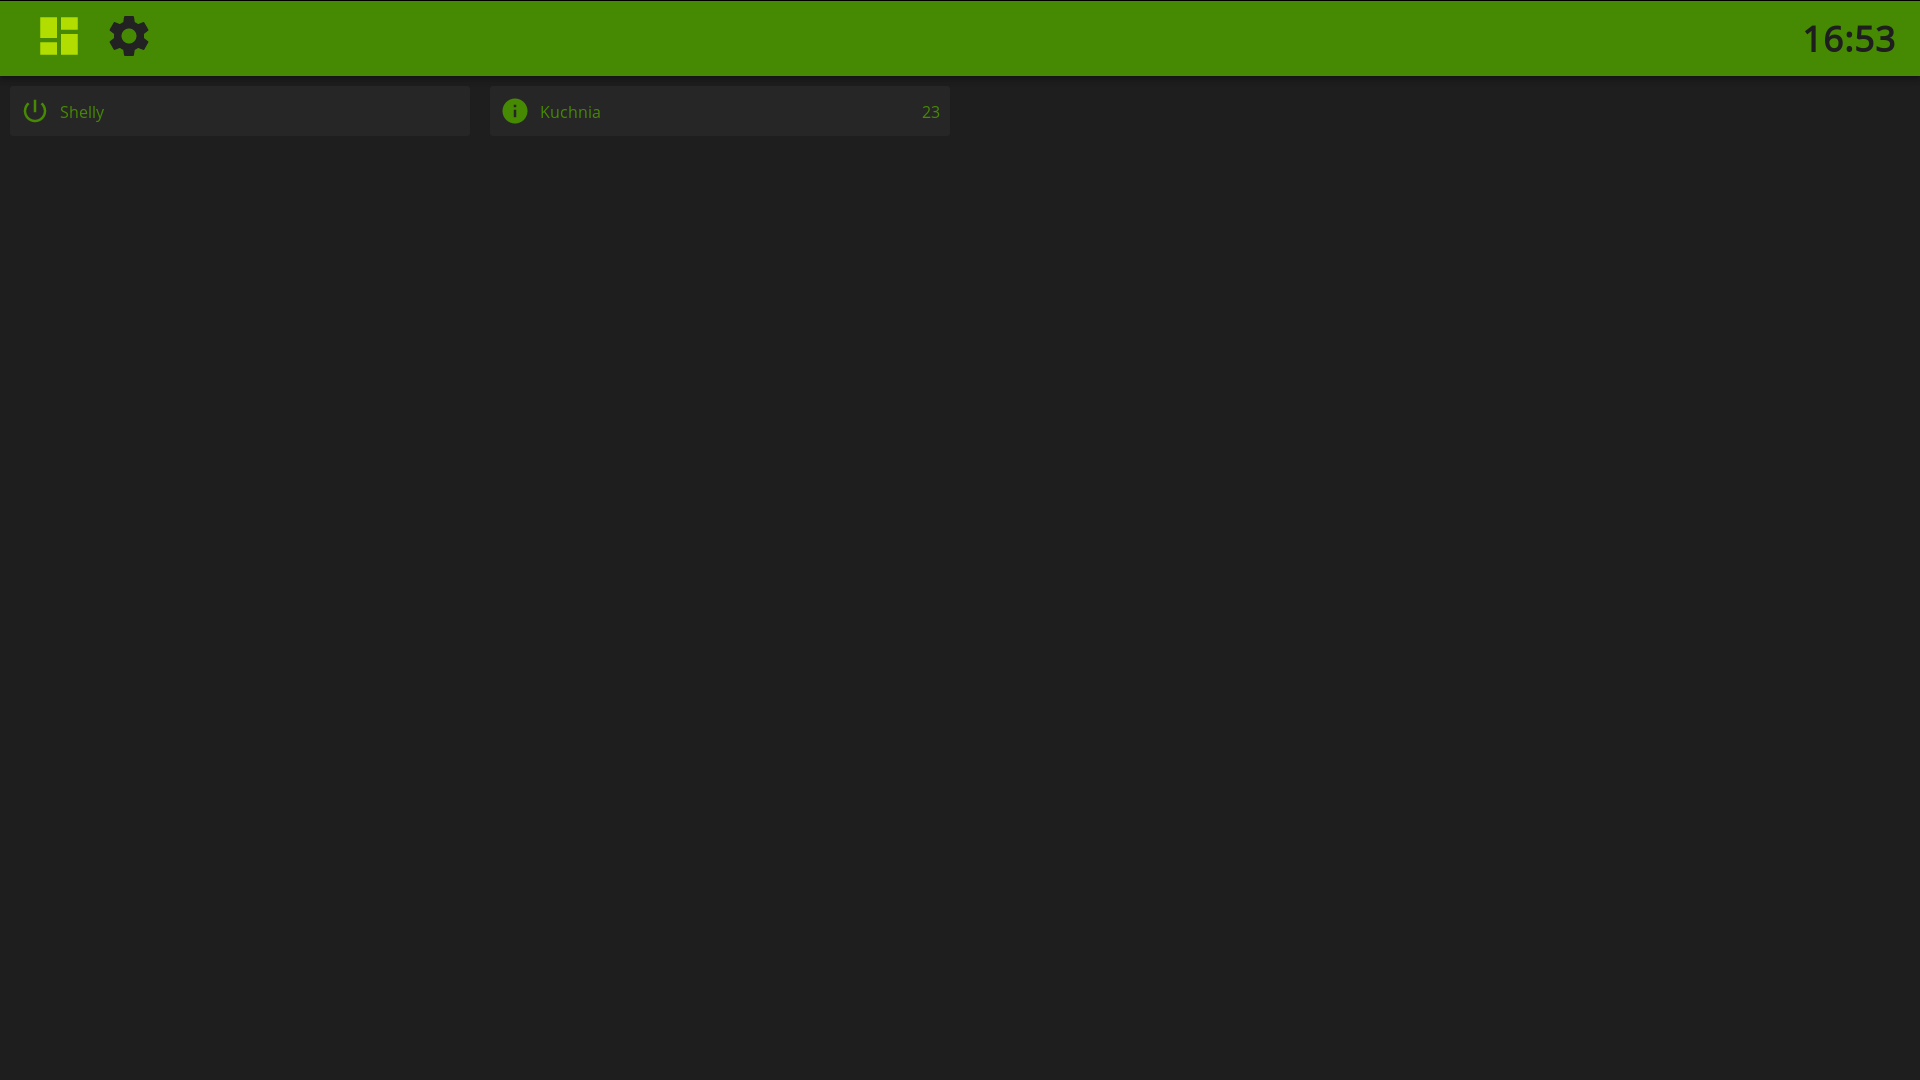
\includegraphics[width=\linewidth]{dashboard.png}
  \caption{Dashboard}
  \label{fig:dashboard}
\end{figure}
\newpage

\subsection{Settings}
Strona służy do konfiguracji naszego systemu. Istnieje tutaj możliwość dodania nowych urządzeń, edycji już istniejących lub wglądu do szczegółów takich jak logi urządzeń.
\begin{figure}[h!]
  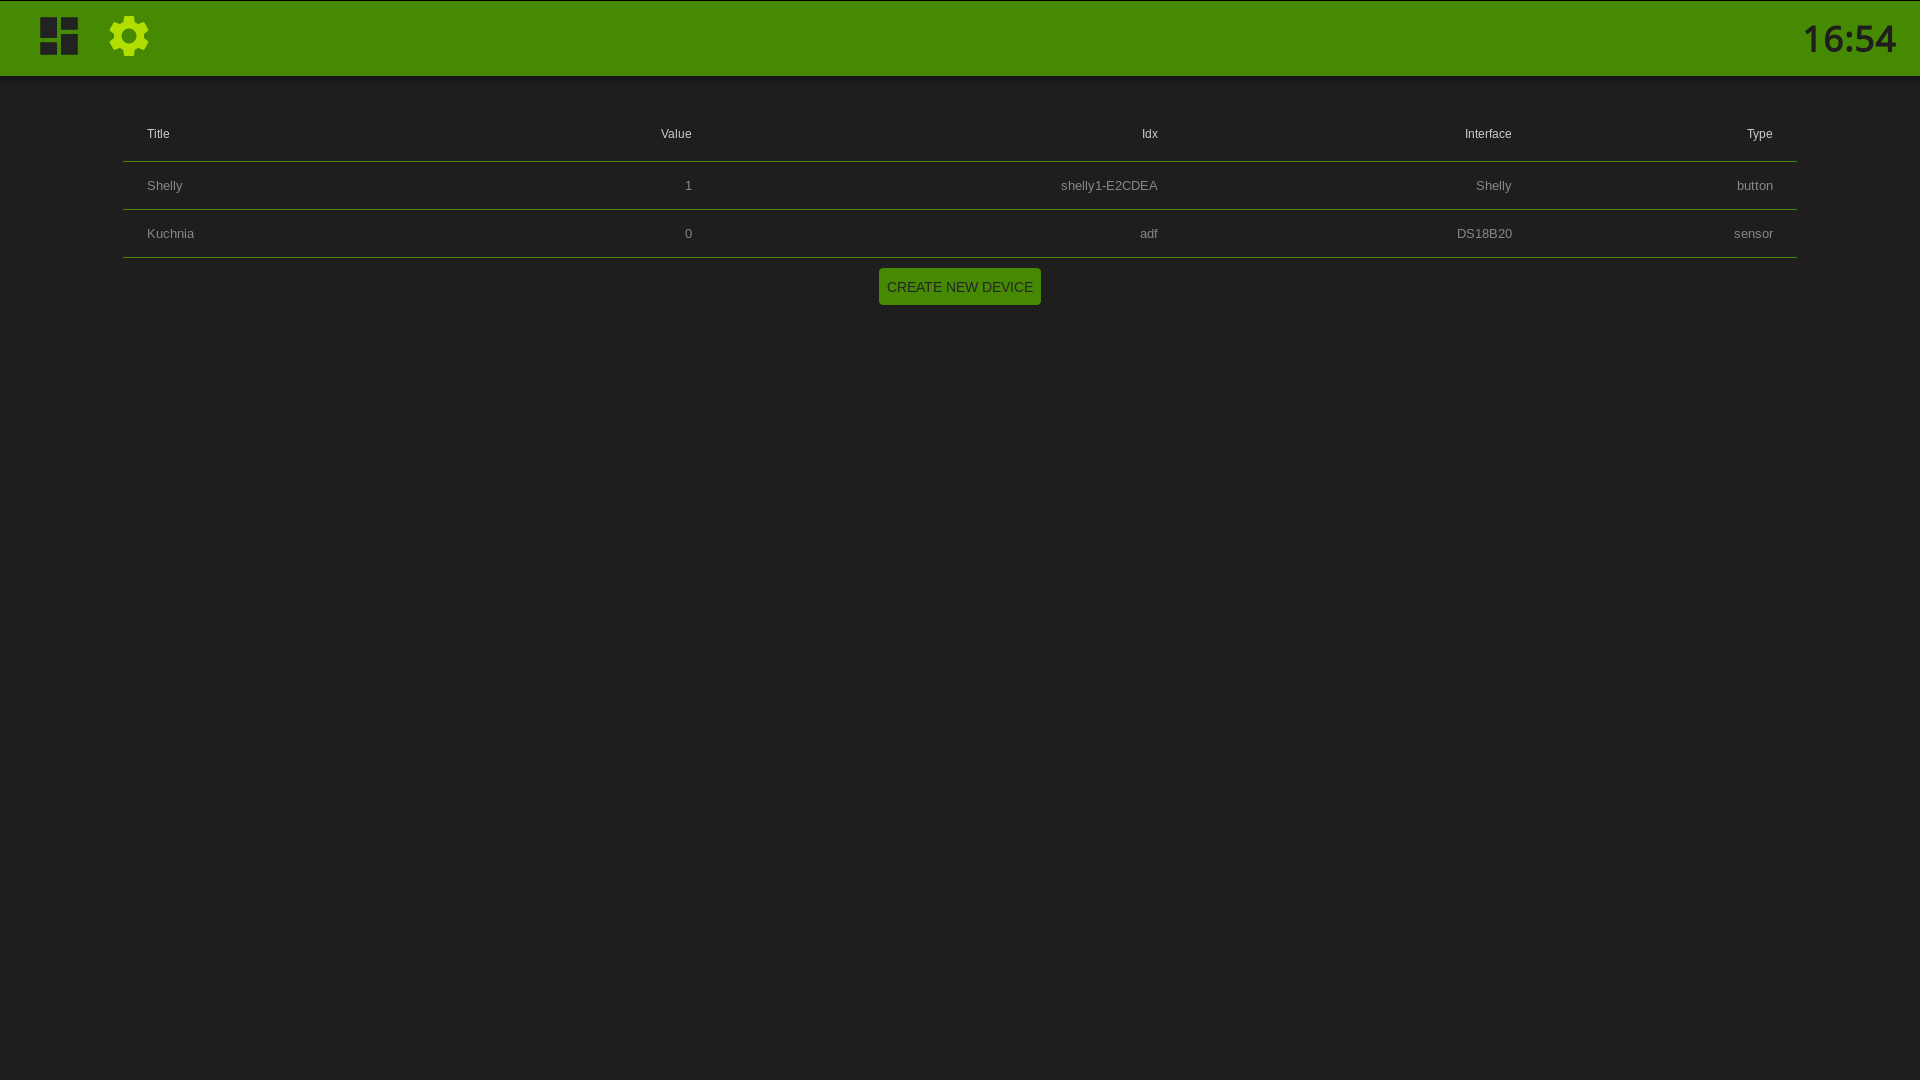
\includegraphics[width=\linewidth]{settings.png}
  \caption{Settings}
  \label{fig:settings}
\end{figure}
\newpage
\section{Serwer}
Serwer jest pośrednikiem między poleceniami użytkownika, a urządzeniami. Jednocześnie zapisuje aktualną konfigurację w bazie danych i trzyma logi. Jest on podzielony na komponenty:
\begin{itemize}
    \item http,
    \item baza danych,
    \item API do urządzeń.
\end{itemize}
Został on napisany w języku javascript. Korzysta on z transpilera babel-node w celu pracy w wersjach es6+. Serwer posiada dodatkowe testy, które sprawdzają działanie niektórych komponentów.
\subsection{HTTP}
Serwer korzysta z obszernego framework'a Express \cite{express} przeznaczonego dla języka javascript, który pozwala zaimportować cały katalog zawierający stronę (listing \ref{lst:http} \ref{lst:connectPublicCat}). Zbudowana strona jest przechowywana w katalogu \textit{public}.\\
Oprócz tego obsługiwane jest wspominane już zapytanie o port, na którym działa websocket (listing \ref{lst:websocket} \ref{lst:getWSPort}).
Ten krótki kod w \ref{lst:http} pokazuje całą strukturę http w projekcie.
\begin{lstlisting}[columns=fullflexible,caption={http.js}\label{lst:http},language=Java]
export const listen = config => {
    app.get('/websocket_port', (req, res) => {
        res.json({port: config.WS_PORT}) /*!\annotation{lst:getWSPort}!*/
    })
    app.use(express.static(config.HTMLPath)); /*!\annotation{lst:connectPublicCat}!*/
    app.get('/', (req, res) => {
        res.sendFile(`${config.HTMLPath}/index.html`);
    });
    app.listen(config.HTTP_PORT, () => console.log(`http listening on port ${config.HTTP_PORT}`))
}
\end{lstlisting}
\subsection{Baza Danych}
Jako, że w założeniach projektu zostało postanowione, że powinien on działać na wielu sprzętach, to użyta została relacyjna baza danych na silniku SQLite \cite{sqlite}. Sama baza nie jest rozbudowana i zawiera tylko dwie tabele czyli logi i urządzenia. Czas w logach jest typu int, mimo że SQLite posiada typ danej timestamp. Powodem tej decyzji jest łatwiejsza integracja ze środowiskiem javascript \cite{sqlitejs}.
\begin{figure}[h!]
  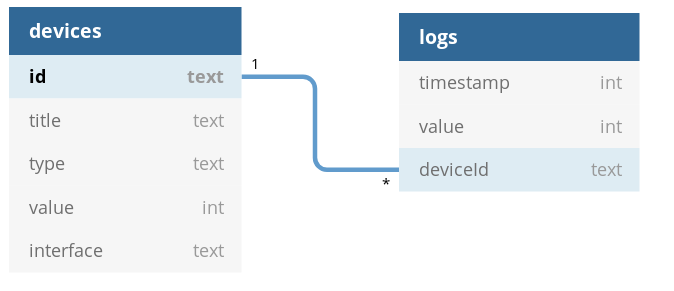
\includegraphics[width=\linewidth]{db.png}
  \caption{schemat bazy}
  \label{fig:db}
\end{figure}

Obsługa bazy danych ma przewidziany osobny moduł w serwerze, który upraszcza wiele procesów. W listingu \ref{lst:updateDeviceSQL} została zaprezentowana funkcja do aktualizacji urządzeń w bazie. Posiada ona tylko jeden argument, którym jest urządzenie do zaktualizowania (listing \ref{lst:updateDeviceSQL} \ref{lst:updateDeviceParameter}) Dzięki temu funkcja może być łatwo re-używalna w przypadku integracji nowych urządzeń i pisania do nich komponentów. Funkcja ta buduje komendę SQL (listing \ref{lst:updateDeviceSQL} \ref{lst:updateDeviceBuildCommand}), a następnie dodaje nowy log (listing \ref{lst:updateDeviceSQL} \ref{lst:updateDeviceAddNewLog})  w przypadku gdy wartość urządzenia uległa zmianie (na przykład zmieniła się temperatura).
\newpage
\begin{lstlisting}[columns=fullflexible,caption={edycja urządzenia}\label{lst:updateDeviceSQL},language=Java]
export const updateDevice = (device) => { /*!\annotation{lst:updateDeviceParameter}!*/
	return new Promise(async (resolve, reject) => {
		let command = `UPDATE ${tables.DEVICES} SET`;
		Object.keys(device).forEach(
		    (key)=>key!=='id' && (command+=` ${key}="${device[key]}",`)); /*!\annotation{lst:updateDeviceBuildCommand}!*/
		command = command.slice(0, -1);
		command += ` WHERE id="${device.id}"`;
		const shouldPushLog = await checkIfValueChanged(device);
		if (shouldPushLog) {
			addNewLog(device); /*!\annotation{lst:updateDeviceAddNewLog}!*/
		}

		db.run(command, (err, result) => {
			if (err) {
				console.error(err);
				reject();
			}
			resolve();
		});
	});
};
\end{lstlisting}
Charakter działania wygląda podobnie przy reszcie funkcji z tego modułu, dzięki czemu użytkownik nie potrzebuje wiedzy o strukturze bazy danych w celu korzystania z niej. 

\subsection{MQTT}
Serwer posiada obsługę MQTT w celu komunikacji z urządzeniami automatyki. W ramach projektu zintegrowany został sterownik przekaźnikowy Shelly1, który jest sterowany za pomocą tego protokołu. Moduł ten został napisany w osobnym pliku, a program \textit{mossquitto} pełni funkcję brokera.
\par \ref{lst:initMQTT} pokazuje jedyny spójny element dla każdego modułu wykorzystujący MQTT. W rozdziale 6 została opisana implementacja API w projekcie.

\begin{lstlisting}[columns=fullflexible,caption={inicializacja modułu mqtt}\label{lst:initMQTT},language=Java]
try {
	exec('mosquitto -p 27007', (error, stdout, stderr) => {
		if (error) {
			console.error(error);
		}
	});
} catch (err) { console.log(err) }
\end{lstlisting}

\chapter{Przykłady działania}
W trakcie prac został podłączony po MQTT sterownik przekaźnikowy, który sterował lampką oraz czujnik temperatury DS18B20 do platformy, która działała na urządzeniu Raspberry Pi oraz na laptopie. Płytka Raspberry została wykorzystana z kilku względów. 
\begin{itemize}
    \item Małe rozmiary dzięki którym łatwiej nam znaleźć dedykowane stałe miejsce.
    \item Małe zapotrzebowanie na energie, które ma bardzo duży wpływ w przypadku gdy urządzenie działa 24 godziny na dobę.
    \item Mała cena, która wynosi ok 200 zł za wersje 3B+.
\end{itemize}
Oczywiście to urządzenie ma dwie spore wady.
\begin{itemize}
    \item Mała stabilność, która jest efektem tego, że system działa na karcie SD.
    \item Do tego urządzenia musimy sami dostarczyć zasilanie 5V o minimalnym natężeniu 2A. Często z winy słabej jakości kabla albo zasilacza awaryjność powoduje, że musimy restartować urządzenie raz na miesiąc czy nawet na tydzień.
\end{itemize}
Warto jednak tutaj wspomnieć jednak że użytkownicy raspberry instalują system na dysku ssd co znacznie wydłuża żywotność i przy lekkich platformach system potrafi pracować wiele lat bez przerwy spowodowanej awarią. Eliminuje to nam pierwszą wadę urządzenia lecz można się z tym raczej spotkać tylko w hobbistycznych projektach, a nie w komercyjnych rozwiązaniach.
\par
Wady i zalety pokazują, że jest to świetna konfiguracja prototypownia, a nie do długoterminowej instalacji. Jako że grupa docelowa tej platformy głównie korzysta z tego urządzenia to postanowiłem na nim stworzyć przykładową implementację.
\newpage
\section{Shelly}
Najbardziej kosztownym czasowo punktem było zintegrowanie platformy ze sterownikiem Shelly1 który może być sterowany przez protokół mqtt. 
\begin{figure}[h]
  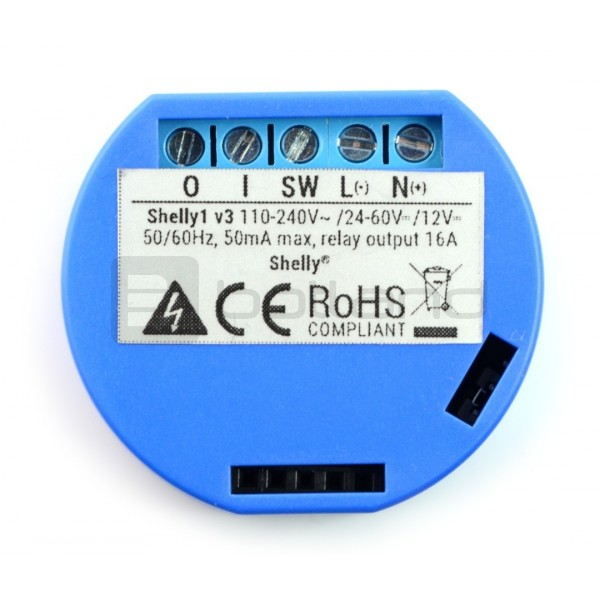
\includegraphics[width=\linewidth]{shelly1.jpg}
  \caption{Shelly1}
  \label{fig:shelly}
\end{figure}
API jest udostępnione na stronie producenta i praca polegała na zintegrowaniu sterownika z serwerem.
API dla sterownika Shelly1 wygląda następująco:
\begin{itemize}
    \item shellies/<model>-<deviceid>/relay/0 by zareportować \textit{on} lub \textit{off}
    \item shellies/<model>-<deviceid>/relay/0/command akceptuje \textit{on} lub \textit{off}
    \item shellies/<model>-<deviceid>/input/0 reportuje stan wejścia SW
    \item shellies/<model>-<deviceid>/longpush/0 reportuje stan długiego wciśnięcia jako 0 lub 1
\end{itemize}
dochodzi jeszcze jeden ogólny kanał dla każdego modelu \textit{shellies/announce} na którym "przedstawia się" każdy nowo podłączony sterownik.
\begin{lstlisting}[columns=fullflexible,caption={sterowanie shelly}\label{lst:shelly},language=Java]
export const setRelay = (id, state) => {
	client.publish(`shellies/${id}/relay/0/command`, state);
};


client.on('message', (topic, message) => {
	if (topic === 'shellies/announce') {
		const announcement = JSON.parse(message.toString());
		console.log('new shelly: ', announcement.id);
		shellies[announcement.id] = { ip: announcement.ip };
	} else {
		const id = topic.split('/')[1];
		const prop = topic.split('/')[2];
		messageHandler(id, prop, message.toString());
	}
});
\end{lstlisting}
\section{DS18B20}
\chapter{Podsumowanie}
\label{chap:podsumowanie}
Celem pracy było stworzenie oprogramowania wspierającego automatykę budynkową. Założenia tego projektu to elastyczność pod względem łączonych urządzeń i pod względem systemu na jakim działa. 
Łatwa konfiguracja i implementacja nowych urządzeń
Łatwy i szybki dostęp do sterowania dla użytkowników budynku.
Założenia zostały spełnione co zostało pokazane w przykładowej implementacji.
\newline
Stworzona platforma jest jeszcze pełna niedoskonałości i na rynku istnieją lepsze systemy, lecz podstawowe cele zostały spełnione i technicznie jest to oprogramowanie gotowe do implementacji i użytku. Zostało to udowodnione na przykładowej implementacji która pokazuje wartość tego oprogramowania. Program został stworzony przy pomocy nowoczesnych technologii i praktyk. W celu dalszego rozwoju tego produktu warto rozważyć następujące sprawy:
\begin{itemize}
    \item Poprawa UI/UX
    \item refactoring kodu
    \item wsparcie większej ilości urządzeń
    \item wsparcie większej ilości inteface'ów
    \item stworzenie narzędzi do łatwiejszej implementacji dla ludzi bez wiedzy programistycznej (Na przykład dla elektryków).
    \item zabezpieczenie panelu przed niepowołanymi ludźmi
    \item poprawa aktualnych błędów i dodawanie dodatkowych funkcjonalności dla poprawy wygody użytkowników
\end{itemize}
Jako że istnieje kilka rozbudowanych i darmowych platform to sens ekonomiczny tego projektu jest znikomy. Warto rozważyć hostowanie platformy dla klientów by nie musieli inwestować w domowy serwer lub mała jednorazowa opłata dla użytku własnego lecz wtedy powinniśmy ograniczyć ingerencję w kod. 

%\bibliographystyle{plalpha}
\bibliographystyle{plabbrv}

%UWAGA: bibliotekę referencji należy przygotować samemu. Dobrym do tego narzędziem jest JabRef.
%       Nazwę przygotowanej biblioteki wpisuje się poniżej bez rozszerzenia 
%       (w tym przypadku jest to "dokumentacja.bib")
\nocite{*}
\bibliography{dokumentacja}
\appendix

\chapterstyle{noNumbered}
\phantomsection % sets an anchor
% \addcontentsline{toc}{chapter}{Indeks rzeczowy}
\printindex

\end{document}
